\section{Evaluation}
\label{sec:evaluation}

For reference, Accuracy is defined as:

\begin{equation}
    \label{eq:Equation17}
    \dfrac{TP + TN}{TP + FP + TN + FN}
\end{equation}

Precision is defined as:

\begin{equation}
    \label{eq:Equation18}
    \dfrac{TP}{TP + FP}
\end{equation}

Recall is defined as:

\begin{equation}
    \label{eq:Equation19}
    \dfrac{TP}{TP + FN}
\end{equation}

F1-Score is defined as:

\begin{equation}
    \label{eq:Equation20}
    \dfrac{2\eqref{eq:Equation18}\eqref{eq:Equation19}}{\eqref{eq:Equation18} + \eqref{eq:Equation19}} = \dfrac{TP}{TP + \frac{1}{2}(FP + FN)}
\end{equation}

Where:
\begin{itemize}
    \item $TP$ is the count of where both predictions and true values are positive
    \item $FP$ is the count of where predictions are positive but true values are negative
    \item $TN$ is the count of where both predictions and true values are negative
    \item $FN$ is the count of where predictions are negative but true values are positive
\end{itemize}

\subsection{Logistic Regression}
\label{sec:evaluation:Logistic Regression}
After running the logistic regression file multiple times, we noticed that the results for each situation between each run were very similar. So, we decided to include the results from one run to maintain space. On the left-hand side of Table \ref{tab:Table1}, you can see the different experiment setting each logistic regression model created. Table \ref{tab:Table1} shows the accuracy, precision, recall and F1-measure results. The accuracy for the Logistic Regression Built in function was around 81.74\%. All the models worked well in terms of accuracy, but the one that came the closest was the ones that involved k-fold cross validation. These tests almost always had an 80\% or higher accuracy rate. The same could be said for precision and F1-measure. However, for recall, the models without k-fold cross validation had a more similar result to the built in function, which was around 85\%.\\

\noindent Between Batch gradient descent and stochastic gradient descent, there wasn’t that much of a difference in the results. They were either the same percentage, or off by 1 point. K-Fold Cross Validation seems to have a huge effect in making the model more precise. It is very clear in these results that it’s better to do k-fold cross validation than not in order to get more accurate results. This makes sense, since it creates multiple training groups and can create a better model as a result of this.\\

\noindent Table \ref{tab:Table2} shows the True Positive, False Positive, True Negative and False Negative Results for the Logistic Regression Model in the different experimental settings.

\begin{table}[ht]
    \centering
    \begin{tabular}{|l|l|l|l|l|}
        \hline
        \textbf{Algorithm}                   & \textbf{Accuracy} & \textbf{Precision} & \textbf{Recall} & \textbf{F1-Score} \\
        \hline
        \textbf{Batch Gradient Descent}      & 77.625            & 73.546             & 86.827          & 79.637            \\
        \textbf{Stochastic Gradient Descent} & 77.999            & 74.397             & 85.899          & 79.736            \\
        \textbf{K-Folds = 5 (BGD)}           & 80.905            & 77.929             & 86.259          & 81.876            \\
        \textbf{K-Folds = 5 (SGD)}           & 80.864            & 77.655             & 86.662          & 81.910            \\
        \textbf{K-Folds = 10 (BGD)}          & 80.936            & 77.718             & 86.779          & 81.972            \\
        \textbf{K-Folds = 10 (SGD)}          & 81.440            & 77.968             & 87.695          & 82.523            \\
        \textbf{Sci-Kit Learn}               & 81.739            & 79.988             & 85.034          & 82.434            \\
        \hline
    \end{tabular}
    \caption{Metrics of Different Algorithms (Averaged)}
    \label{tab:Table1}
\end{table}

\begin{table}[ht]
    \centering
    \begin{tabular}{|l|l|l|l|l|}
        \hline
        \textbf{Algorithm}                   & \textbf{TP} & \textbf{FP} & \textbf{TN} & \textbf{FN} \\
        \hline
        \textbf{Batch Gradient Descent}      & 1404        & 505         & 1087        & 213         \\
        \textbf{Stochastic Gradient Descent} & 1389        & 478         & 1114        & 228         \\
        \textbf{K-Folds = 5 (BGD)}           & 838.6       & 237.6       & 734.2       & 133.6       \\
        \textbf{K-Folds = 5 (SGD)}           & 842.6       & 242.4       & 729.4       & 129.6       \\
        \textbf{K-Folds = 10 (BGD)}          & 421.6       & 121         & 365.1       & 64.3        \\
        \textbf{K-Folds = 10 (SGD)}          & 426.1       & 120.5       & 365.5       & 59.9        \\
        \hline
    \end{tabular}
    \caption{Confusion Matrix Results (Averaged)}
    \label{tab:Table2}
\end{table}

\subsection{SVMs}
\label{sec:evaluation:SVMs}

Similar to the logistic regression script, for multiple runs of the support vector machine (SVM) script, SVM produced statistics that were very similar for multiple runs. Therefore, results from one run are included in Table \ref{tab:Table3}. This table shows the accuracy, precision, recall, and f1-measure for the SVM algorithm and the built in SVM function. Table \ref{tab:Table4} shows the True Positive, False Positive, True Negative and False Negative Results for the SVM model.

\begin{table}[ht]
    \centering
    \begin{tabular}{|l|l|l|l|l|}
        \hline
        \textbf{Algorithm}     & \textbf{Accuracy} & \textbf{Precision} & \textbf{Recall} & \textbf{F1-Score} \\
        \hline
        \textbf{SVM}           & 78.218            & 74.931             & 84.625          & 79.483            \\
        \textbf{Sci-Kit Learn} & 82.674            & 78.308             & 90.25           & 83.856            \\
        \hline
    \end{tabular}
    \caption{Metrics}
    \label{tab:Table3}
\end{table}

\begin{table}[H]
    \centering
    \begin{tabular}{|l|l|l|l|l|}
        \hline
        \textbf{Algorithm}     & \textbf{TP} & \textbf{FP} & \textbf{TN} & \textbf{FN} \\
        \hline
        \textbf{SVM}           & 1354        & 453         & 1156        & 246         \\
        \textbf{Sci-Kit Learn} & 1444        & 400         & 1209        & 156         \\
        \hline
    \end{tabular}
    \caption{Confusion Matrix Results}
    \label{tab:Table4}
\end{table}

\subsubsection{Precision-Recall Curves}
\label{sec:evaluation:SVMs:Precision-Recall Curves}

Figures \ref{fig:Figure5} and \ref{fig:Figure6} plot the precision (y-axis) against the recall (x-axis).

\begin{figure}[ht]
    \centering
    \begin{subfigure}[t]{.45\textwidth}
        \centering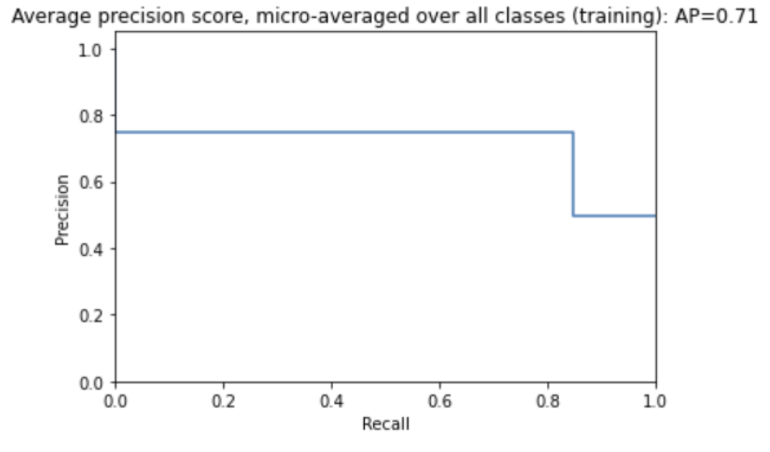
\includegraphics[width=1\linewidth]{PR1}
        \caption{PR Curve of Our Model}
        \label{fig:Figure5}
    \end{subfigure}
    \begin{subfigure}[t]{.45\textwidth}
        \centering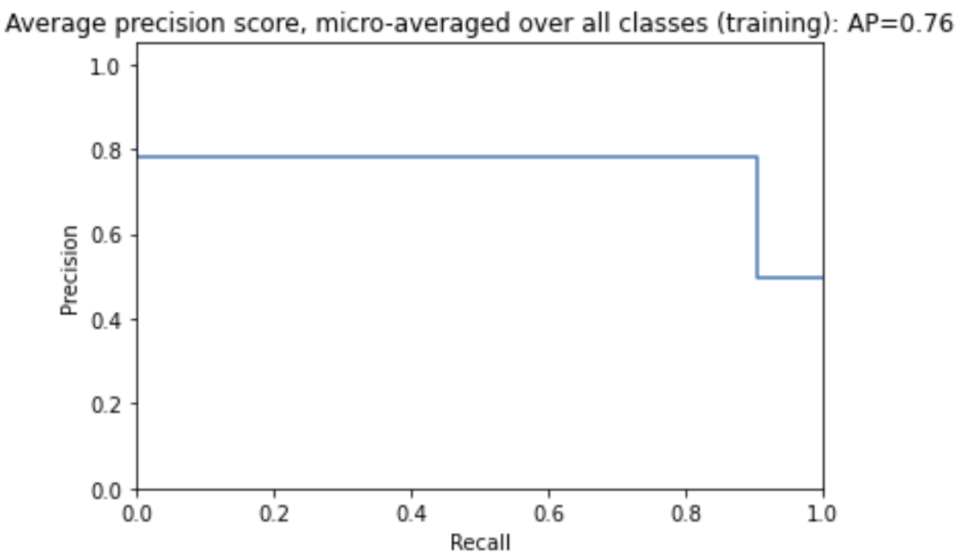
\includegraphics[width=1\linewidth]{PR2}
        \caption{PR Curve of Sci-Kit Learn's Model}
        \label{fig:Figure6}
    \end{subfigure}
\end{figure}

\subsection{Random Forest}
\label{sec:evaluation:Random Forest}

Unlike Logistic Regression and SVMs, our Random Forest model was somewhat flawed as we assumed all data was continuous rather than looking at a mix of continuous and discrete data. Due to this, not was our DT model unnecessarily expensive in both time and space complexities, but it caused our Random Forest model to be not much of an improvement over a regular DT. Table \ref{tab:Table5} and Table \ref{tab:Table6} show the results of ID3 and Random Forest:

\begin{table}[ht]
    \centering
    \begin{tabular}{|l|l|l|l|l|}
        \hline
        \textbf{Algorithm}     & \textbf{Accuracy} & \textbf{Precision} & \textbf{Recall} & \textbf{F1-Score} \\
        \hline
        \textbf{ID3}           & 70.365            & 65.722             & 86.085          & 74.538            \\
        \textbf{Sci-Kit Learn} & 89.685            & 88.503             & 91.404          & 89.93             \\
        \hline
    \end{tabular}
    \caption{ID3 Metrics}
    \label{tab:Table5}
\end{table}

\begin{table}[ht]
    \centering
    \begin{tabular}{|l|l|l|l|l|}
        \hline
        \textbf{Algorithm}     & \textbf{Accuracy} & \textbf{Precision} & \textbf{Recall} & \textbf{F1-Score} \\
        \hline
        \textbf{Random Forest} & 71.206            & 66.651             & 85.776          & 75.014            \\
        \textbf{Sci-Kit Learn} & 94.734            & 93.773             & 95.918          & 94.833            \\
        \hline
    \end{tabular}
    \caption{Random Forest Metrics}
    \label{tab:Table6}
\end{table}